\documentclass[letterpaper,11pt]{article}
\oddsidemargin -1.0cm \textwidth 17.5cm

\usepackage[utf8]{inputenc}
\usepackage[activeacute,spanish]{babel}
\usepackage{amsfonts,setspace}
\usepackage{amsmath}
\usepackage{amssymb, amsmath, amsthm}
\usepackage{comment}
\usepackage{amssymb}
\usepackage{dsfont}
\usepackage{anysize}
\usepackage{multicol}
\usepackage{enumerate}
\usepackage{graphicx}
\usepackage[left=1.5cm,top=2cm,right=1.5cm, bottom=1.7cm]{geometry}
\setlength\headheight{1.5em} 
\usepackage{fancyhdr}
\usepackage{multicol}
\usepackage{hyperref}
\usepackage{wrapfig}
\pagestyle{fancy}
\fancyhf{}
\renewcommand{\labelenumi}{\normalsize\bfseries P\arabic{enumi}.}
\renewcommand{\labelenumii}{\normalsize\bfseries (\alph{enumii})}
\renewcommand{\labelenumiii}{\normalsize\bfseries \roman{enumiii})}

\begin{document}

\fancyhead[L]{\itshape{Facultad de Ciencias F\'isicas y Matem\'aticas}}
\fancyhead[R]{\itshape{Universidad de Chile}}

\begin{minipage}{11.5cm}
    \begin{flushleft}
        \hspace*{-0.6cm}\textbf{FI1000-5 Introducción a la Física Clásica}\\
        \hspace*{-0.6cm}\textbf{Profesora:} Paulina Lira\\
        \hspace*{-0.6cm}\textbf{Auxiliares:} Alejandro Silva, Felipe Kaschel, Juan Cristóbal Castro\\
    \end{flushleft}
\end{minipage}

\begin{picture}(2,3)
    \put(405,-5){\includegraphics[scale=1.25]{2020-1/Imágenes/logo/fcfm2.pdf}}
\end{picture}

\begin{center}
	\LARGE \bf Auxiliar \#5: MCU-MCUA\\
\end{center}


\vspace{-1cm}
\begin{enumerate}\setlength{\itemsep}{0.4cm}

\rfoot[]{pág. \thepage}


\item[]
\item Un mono se encuentra colgado de una rueda que gira horizontalmente con un periodo T, y que está a una altura H, como se indica en la figura. Además el eje sobre el cual gira la rueda esta en el borde de un plano inclinado, de ángulo $\theta$ con la horizontal. El mono se suelta justo cuando va pasando sobre el borde del plano inclinado tal que cae a una distancia D de ese punto. Determine el radio de la rueda.
\begin{figure}[h!]
        \centering
        \includegraphics[scale=0.7]{2020-1/Imágenes/aux5/fig1.pdf}/
\end{figure}

\item Un auto se mueve a velocidad v sobre un trayecto rectilíneo. Si el radio de sus ruedas es R, determine:
\begin{enumerate}
    \item Velocidad angular de las ruedas en torno a su eje.
    \item La aceleración angular si el conductor pisa suavemente el freno y el auto se detiene uniformemente luego de que las ruedas dan N vueltas.
    \item Distancia recorrida si, antes de comenzara frenar, el auto avanza durante $\Delta t$ segundos.
\end{enumerate}
\begin{figure}[h!]
        \centering
        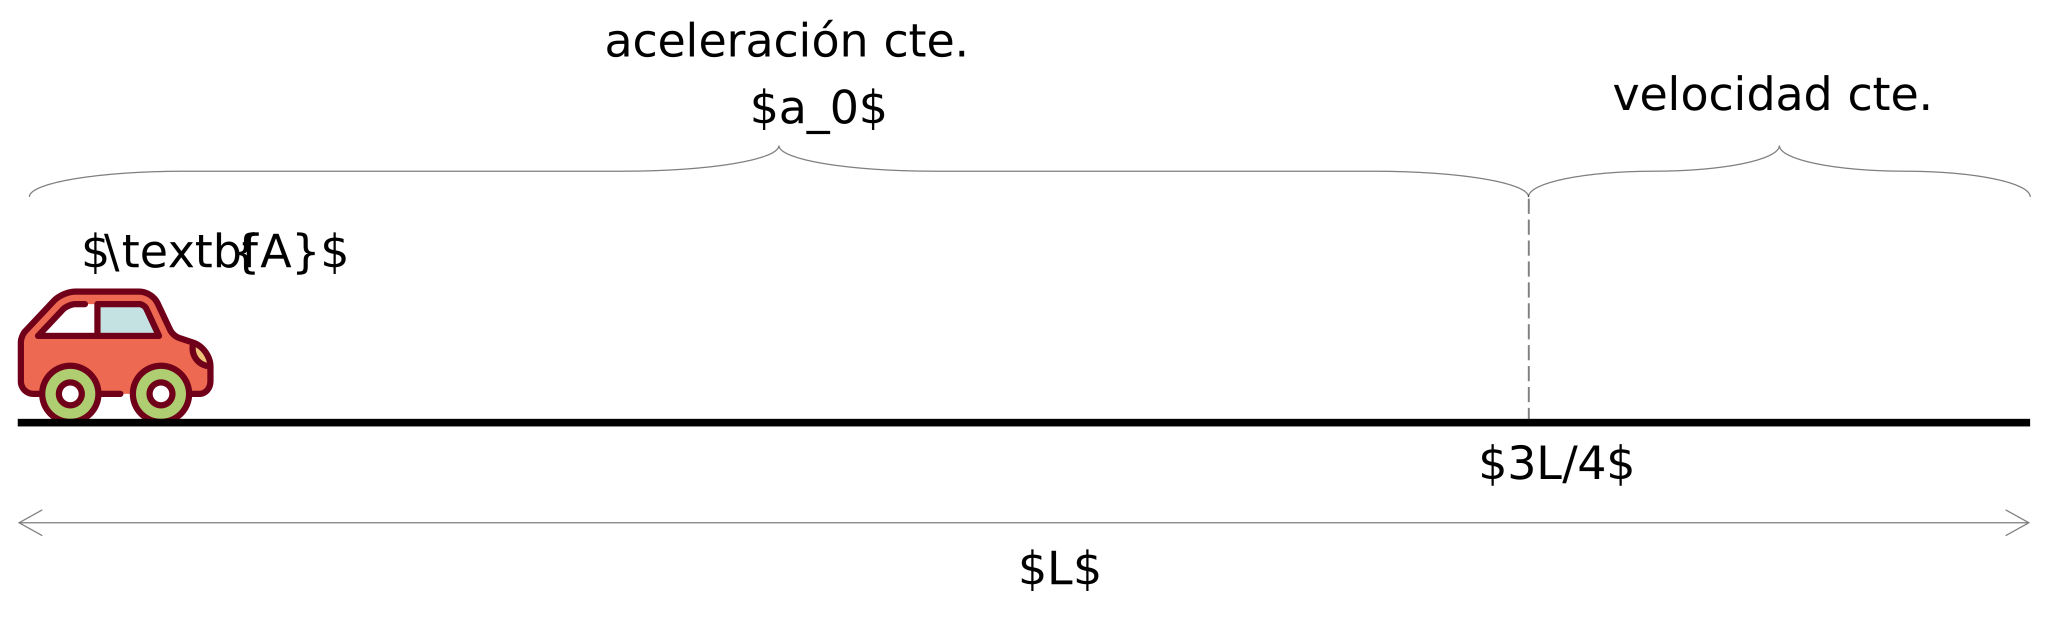
\includegraphics[scale=0.3]{2020-1/Imágenes/aux5/auto.jpg}/
\end{figure}

\end{enumerate}
\end{document}